\chapter{Germanium Detectors}\label{chap:gedet}
Ionizing radiation produces information carriers in matter: electron-ion pairs and electron-hole pairs in gas filled chambers and semiconductor crystals respectively. The thermal excitation of electrons, produces mobile charge carriers (electrons and holes) in semiconductors as well. Impurities in the crystal lattice further contribute to this effect. The presence of these charge carriers masks the electron-hole pairs produced by ionizing radiation. 

A zone depleted of mobile charge carriers -- a \textit{depletion} region -- is needed for particle detection in semiconductors. As will be explored in this chapter, semiconductor properties can be exploited to create these conditions. The depletion region acts as the sensitive, or active, volume of a semiconductor detector and its depth is tied to the impurity levels of the crystal. As discussed in the previous chapter, gammas have attenuation lengths of up to 6\,cm in Ge. To achieve a depletion depth of this order, impurity levels on the order of 1 part per $10^{12}$ are required. This unprecedented impurity level has been achieved in Ge, but not in other semiconductors~\cite{knoll}. 

Germanium detector technology has been developed since the 1960's, finding a natural application in gamma-ray spectroscopy. In addition to the high density and large active volume of Ge detectors, the excellent energy resolution of these devices -- a direct consequence of the low energy needed to create an electron-hole pair in contrast with other information carriers -- makes them attractive for rare-event searches. Ge detectors are prized for their unprecedentedly pure nature, and recent advances in detectors suitable for rare-event searches have pushed their active volumes to multi-kg scales without sacrificing their performance~\cite{icpc,icpc_psd}. The resulting elevated volume-to-surface ratio mitigates backgrounds originating from surface interactions, such as those caused by charged particles external to the detector. This chapter provides a brief overview of the general working principle of germanium detectors, and places emphasis on the Ge detector geometries used for \novbb{} searches. The band structure is at the heart of how semiconductors function. Thus band structure theory is introduced, followed by some its emergent properties: effective mass and mobilities. Mobilities in turn dictate charge drift, which as will be seen in Section~\ref{sec:charge_drift} shape the time profile of a Ge detector signal. 

While this chapter focuses on Ge, the same working principle (Sections~\ref{sec:band_structure}-\ref{sec:charge_drift}) applies to other semiconductor detectors. In recent decades, a new candidate for gamma-ray spectroscopy has emerged. Developments in cadmium-zinc-telluride (CdZnTe or simply CZT) detectors has lead to energy resolutions approaching those of Ge~\cite{delSordo2009}, and depletion regions on the order of 1\,cm thick~\cite{Wahl2015}. Unlike Ge detectors which require cryogenic operating temperatures, CZT detectors can be operated at room temperature, allowing for the design of compact gamma-ray detection modules. In Chapter~\ref{chap:scanner} a device which employs this technology to study Ge detector response is introduced.  


\section{Band Structure of Crystals}\label{sec:band_structure}
In 1929 Felix Bloch theorized that electrons confined in a crystalline lattice with periodic potential $u(\vec{r})$ behave like free electrons but a with periodic modulation given by $u(\vec{r})$. The electron's wavefunction, $\psi(\vec{r})$, thus takes the form:
\begin{equation}
	\psi(\vec{r}) = u(\vec{r})e^{i\vec{k} \cdot \vec{r}}
	\label{eq:bloch}
\end{equation}
where an electron at position $\vec{r}$ has a wavevector $\vec{k}$~\cite{bloch}. These so-called \textit{Bloch functions} are solutions to the time-independent Sch\"odinger equation -- with potential $u(\vec{r})$. A one-dimensional crystal lattice will be used as an example throughout the chapter for illustrative purposes. The basic concepts derived from it apply to 3-dimensional crystal lattices as well.

The one-dimensional crystal lattice potential obeys translational symmetry $u(x)$ = $u(x + a)$, where $a$ is length of a primitive cell of the crystal. The primitive cell is the smallest structure which once repeated and translated recreates the entire crystal. By substituting a Bloch function, $\psi(x)$, into the Sch\"odinger equation and applying the periodic boundary conditions of the reciprocal lattice on $k$, the dispersion relation -- the energy $E$-wavevector relation -- of electrons confined in the crystal lattice can be found. Near a \textit{Brillouin zone} boundary ($k = \frac{1}{2}G$) it can be shown that the dispersion relation is approximated by:
\begin{equation}
	E_e^\pm(k) =  \Gamma \pm U + \frac{\hbar^2\left(k-\frac{1}{2}G\right)^2}{2m_e}\left(1 \pm \frac{2\Gamma}{U}\right)
	\label{eq:dispersion_crystal}
\end{equation}
for $\Gamma/U \ll 1$, where $\Gamma \equiv \hbar\left(\frac{1}{2}G\right)^2/2m_e$, $U \equiv u\left(\frac{1}{2}G\right)$ and $G = 2\pi/a$ is the reciprocal lattice vector~\cite{kittel}. The Brillouin zone is the geometrical analogue of primitive cell in reciprocal lattice space. Note that the dispersion relation of a free electron is given by $E_e(k) = \hbar^2k^2/2m_e$, thus $\Gamma$ is the free electron energy evaluated at the zone boundary. Both dispersion relations are shown in Fig.~\ref{fig:bandgap}.
\begin{figure}[htb]
	\centering
	\includegraphics[width=5in]{figs/ge/band_gap_width_5in.pdf}
	\caption{Dispersion relations of electrons confined to a crystal lattice and free electrons. The dispersion relation for electrons bound to a crystal exhibits a range of forbidden energies of width $E_g$ -- the band gap. For display purposes, the value of $U$ is set artificially high to $U=-\frac{3}{5}\hbar\left(\frac{1}{2}G\right)^2/2m_e =-\frac{3}{5}\Gamma$} 
	\label{fig:bandgap}
\end{figure}

Two energy bands, $E_e^+$ and $E_e^-$, are described by the parabolic approximation of the dispersion relation in Eq.~\ref{eq:dispersion_crystal}. In between these bands no wavelike electron orbitals exist~\cite{kittel}. This region, void of allowed energy levels, is known as the band gap. In semiconductors this gap is of the order of 1\,eV. The band gap has its physical origins in Bragg reflection. When the Bragg condition, $k=n\pi/a$ (commonly stated as a condition on the wavelength $n\lambda = 2d\sin\theta$ with $\theta = \pi/2$ and integer $n$), is met, electron waves incident on and reflected by the crystal lattice interfere forming standing waves. These standing waves have two modes, one which piles up electrons at ion cores and the other in between them. The energy of the first, $E_e^+$, is lower than that of a free electron, whereas the second, $E_e^-$, has a higher energy. Note that $U \le 0$. The energy difference between the bands is given by the band gap, $E_g$, at $k=n\pi/a$.

Given a crystal with $N$ primitive cells, each primitive cell ``contributes exactly one independent value of $k$ to each energy band''~\cite{kittel}. Accounting for electron spin, each energy band has $2N$ orbitals. The parity of the number of electrons in each primitive cell determines if a crystal is an insulator at 0\,K: it is a necessary but insufficient condition that this number be even. The final condition is that the energy bands need not overlap. An even number of valence electrons per primitive cell guaranties that one or more bands will be completely filled. An electron in a filled band does not contribute to the conductivity of a crystal because the filled accessible energy levels impede a continuous change in its momentum~\cite{kittel}. The last filled band is known as the valence band and the empty or partially filled band at higher energy as the conduction band. Given these definitions, in the absence of any excitations only electrons in the conduction band contribute to the conductivity of the crystal. 
\begin{figure}[htb]
	\centering
	\includegraphics[width=6in]{figs/ge/ge_structure.png}
	\caption{Schematic of the face-centered cubic diamond structure of Ge exhibiting tetrahedral covalent bonds as shown from the side (left) and with an isometric view (center). The renders are based on depictions of the crystal structure in Ref.~\cite{kittel}. Atoms on the corners, faces and inside the cube are shown in black, orange and blue respectively. The Ge primitive cell is shown within this cube as a shaded parallelepiped (right). The primitive cell contains two Ge atoms. One from the blue atom contained within its volume and one additional one form the $8\times\frac{1}{8}$ atoms in the corners of the parallelepiped. The Miller indices, $\left<hlk\right>$, are used to represent the lattice vector directions.} 
	\label{fig:ge_structure}
\end{figure}

Crystalline Ge has the face-centered cubic structure of diamond~\cite{kittel}. As exemplified by Fig.~\ref{fig:ge_structure}, there are 2 atoms per primitive cell of a Ge crystal. Each of these atoms has valence 4, which totals 8 valence electrons in the primitive cell. The valence and conduction bands of Ge (shown in Fig.~\ref{fig:band_structure}) do not overlap, therefore Ge -- and similarly, Si -- is an insulator at 0\,K. The four valence bands arise from the hybridization of the triply-degenerate 4p ($l = 1$, $m_l = 0, \pm1$) and the 4s ($l = 0$, $m_l = 0$) orbitals of Ge. Using $\left|l,m_l\right>$ notation, the two topmost valence bands correspond to the $\left|1,\pm1\right>$ states. Due to spin-orbit coupling the $\left|1,0\right>$ state lies at an energy $\Delta_{so}$ bellow. Finally, the $\left|0,0\right>$ state is found at the bottom. Each of these bands in filled with 2 electrons, one from each atom in the primitive cell, multiplied by the number of primitive cells, giving $2N$.
\begin{figure}[htb]
	\centering
	\includegraphics{figs/ge/ge_bands.pdf}
	\caption{The band structure of Ge along the $\left<1\,1\,1\right>$ and $\left<1\,0\,0\right>$ directions. The four valence bands are shaded in gray. The band data was extracted from a raw image in Ref.~\cite{knoll} and denoised with some of the same algorithms applied to Ge signals presented in Chapter~\ref{chap:pipeline} to produce the bands shown here.} 
	\label{fig:band_structure}
\end{figure}

 As opposed to the band gap shown in Fig.~\ref{fig:bandgap}, the maximum of the Ge conduction band and the minimum of the valance band do not align at the same wavevector $\vec{k}$ -- an indirect band gap. If these extrema align, a direct band gap is obtained. For valence electrons to traverse a direct band gap -- a direct transition -- they need to absorb a threshold energy of $E_g$. For indirect transitions, however, they must also obtain a change in wavevector. In the case of Ge, electrons at the maximum of the valence band need a change in wavevector of $\frac{2\pi}{a}\left(\frac{1}{2}\,\frac{1}{2}\,\frac{1}{2}\right)$ to transition, as seen from the band structure in Fig.~\ref{fig:band_structure}. Note that this is a threshold transition, given enough energy, electrons generally transition from any $\vec{k}$-point in the valence band to any $\vec{k}$-point in the conduction band, as long as energy and wavevector conservation is observed.

 The change in wavevector can be obtained by exciting a phonon in the crystal. Therefore, electrons in the valence band need a threshold energy of $E_g + \hbar\Omega$, where $\Omega$ is the angular frequency of the phonon, to traverse an indirect gap. Phonon energies ($\hbar\Omega \approx 0.01-0.03$\,eV) are small compared to $E_g$~\cite{kittel}. Above 0\,K, the electron can absorb a thermal phonon from the crystal, in this case the threshold energy for transition is $E_g - \hbar\Omega$. Examples of $E_g$ at 0\,K and 300\,K can be found in Tab~\ref{tab:band_gaps}. The variation of $E_g$ has its origins in ``crystal lattice expansion and phonon-induced atomic vibrations''~\cite{bandgap_with_t} at higher temperatures.
\begin{table}[tbph]
    \centering
    \caption{Band gaps of various semiconductors at 0\,K and 300\,K. The variation in band gap values for Cd$_{1\text{-}x}$Zn$_{x}$Te corresponds to the ratio of Cd to Zn, with the low and high ends corresponding to the subindex values $x = 0$ and $x = 1$. These values are sourced from Ref.~\cite{cdte_bandgap} and Ref.~\cite{znte_bandgap} respectively. In between $x = 0$ and $x = 1$ the Cd$_{1\text{-}x}$Zn$_{x}$Te band gap grows in a non-linear manner~\cite{cdznte_bandgap}. All other values are taken from Ref.~\cite{knoll}.}
    \vspace{12pt}
    \begin{tabularx}{1\textwidth}{>{\tr}X >{\tr}X >{\tr}X >{\tr}X}
		\hline \noalign{\vskip 1ex}
        Crystal & Gap & $E_g$ in eV at 0\,K & $E_g$ in eV at 300\,K \\[1ex]
		\hline \noalign{\vskip 1ex}
        Ge   & indirect & 0.746 & 0.665\\
        Si   & indirect & 1.165 & 1.115\\
        Cd$_{1\text{-}x}$Zn$_{x}$Te  & direct & 1.606 - 2.31 & 1.51 - 2.25\\[1ex]
		\hline
    \end{tabularx}
	\label{tab:band_gaps}
\end{table}

\section{Holes, Effective Mass and Mobility}\label{sec:eff_mass}
When an electron transitions to the conduction band, a vacant orbital is formed in the valence band. This vacancy is referred to as a hole. A hole is the physical interpretation of the missing electron and as will be seen, can be treated as a positive charge carrier. 

If the top of the valence band is used as a zero-energy point, the dynamics of the hole can be understood as a reflection of the valence band over the origin in $k$-space: $E_h = -E_e$ and $\vec{k}_h = - \vec{k}_e$, where $h$ and $e$ denote the hole and missing valence electron respectively. From this inversion over the origin, it follows that the group velocities -- given by $\vec{\text{v}} = \vec{\nabla}_kE/\hbar$ -- of missing electrons and holes are equal. The charge of a hole, $q_h$, can be derived from its equation of motion in an electromagnetic field: 
\begin{equation}
	\hbar \frac{d\vec{k}_h}{dt} = q_h\left(\vec{\mathcal{E}} + \vec{\text{v}}_h\times\vec{\mathcal{B}}\right)~,
	\label{eq:em_force}
\end{equation}
where $\vec{\mathcal{E}}$ and $\vec{\mathcal{B}}$ are the electric and magnetic fields. By applying $\vec{k}_h = - \vec{k}_e$ and  $\vec{\text{v}}_h = \vec{\text{v}}_e$, it is deduced that a hole acts as a positive charge carrier with $q_h = e$. Holes can change their momentum continuously -- by swapping positions in k-space with occupied electron energy levels -- and thus contribute to the conductivity of the crystal. 

From this point forward the discussion will focus on \textit{mobile} charge carriers, that is charge carriers that contribute to the conductivity in a crystal -- conduction electrons and valence holes, to be denoted by the subscripts $e$ and $h$ respectively. Mobile charge carriers behave as free particles in the crystal; however, the lattice imposes its effect by changing the apparent mass of these particles. Although their real mass remains the same, they behave in an electromagnetic field as if imparted with an \textit{effective} mass dictated by the band structure of the crystal.
 
%The curvature of the bands in Fig.~\ref{fig:bandgap} is tied to the mass of the electron and the ratio of the free electron energy at the zone boundary and the width of the band gap: $\Gamma/E_g$. 
The second derivative of the free electron dispersion relation is given by $\frac{d^2E_e}{dk^2} = \frac{\hbar^2}{m_e}$. Generalizing this statement to any dispersion relation in one dimension, the effective mass, $m^*$, is defined as:
\begin{equation}
	\frac{1}{m^*} = \frac{1}{\hbar^2}\frac{d^2E}{dk^2}~.
	\label{eq:effective_mass}
\end{equation}
Applying the definition above to Eq.~\ref{eq:dispersion_crystal}, the effective mass of electrons near the minimum of the conduction band and holes near the maximum of the valence band is obtained for the linear lattice example. These are given by Eq.~\ref{eq:eff_mass_e} and Eq.~\ref{eq:eff_mass_h} respectively.
\vspace{-0.5\baselineskip}
\begin{multicols}{2}
	\begin{equation}
		m_{e}^* = m_e\left(\frac{4\Gamma}{E_g} + 1\right)^{-1}
	\label{eq:eff_mass_e}
	\end{equation}

	\begin{equation}
		m_{h}^* = m_e\left(\frac{4\Gamma}{E_g} - 1\right)^{-1}
	\label{eq:eff_mass_h}
	\end{equation}
\end{multicols}
\noindent In the regime where Eq.~\ref{eq:dispersion_crystal} is valid, $m_e^*$ and $m_h^*$ increase monotonically with increasing $E_g$. Note that the positive hole effective mass near the top of the valence band implies a negative electron effective mass. In practice, this means that when an electric field is applied to such an electron, the momentum transfer from the electron to the lattice will be larger than that of the applied force to the electron~\cite{kittel}.

The effective mass definition of Eq.~\ref{eq:effective_mass} is easily generalized to three dimensions. This extension is necessary for anisotropic band structures such as that of Ge.
\begin{equation}
	\left(\frac{1}{m^*}\right)_{ij} = \frac{1}{\hbar^2}\frac{d^2E}{dk_i dk_j}
	\label{eq:effective_mass_3d}
\end{equation}
Effective mass can be determined experimentally with cyclotron resonance measurements. The measured effective masses of electrons in Ge at the conduction band minimum at $\vec{k} = \frac{2\pi}{a}\left(\frac{1}{2}\,\frac{1}{2}\,\frac{1}{2}\right)$ parallel and perpendicular to the $\left<1\,1\,1\right>$-direction are $(1.64 \pm 0.03)m_e$ and $(0.0819 \pm 0.0003)m_e$ respectively~\cite{eff_mass_e}. The two topmost valence bands at $\vec{k} = \left(0\,0\,0\right)$ correspond to light and heavy holes with effective masses of $0.043m_e$ and $0.34m_e$ respectively~\cite{kittel}.

Mobile charge carriers respond to an electric field as a free particle with mass, $m^*$, until they collide for another particle. The concept of \textit{mobility} accounts for the collisional effects in the lattice and absorbs the effective mass dependence of the equations of motion. By integrating the equation of motion of a charge $q$ in an electric field, $\vec{\mathcal{E}}$,  over a time interval, $\tau$, with no collisions, an expression for the drift velocity, $\vec{v}$, is obtained:
\begin{equation}
	\vec{v} = \frac{q\tau}{m^*}\vec{\mathcal{E}}~.
 	\label{eq:drift_vel}
\end{equation}
The time with no collisions, $\tau$, is referred to as the collision time. On crystal axes (constant $m^*$), holes drift in the same direction as the electric field and electrons in the opposite direction. The absolute value of the proportionality constant in Eq.~\ref{eq:drift_vel} is the aforementioned mobility, defined as the magnitude of drift velocity per unit electric field: 
\begin{equation}
	\mu \equiv v/\mathcal{E}~,
	\label{eq:mobility}
\end{equation}
where $v = \left|\vec{v}\right|$ and $\mathcal{E} = \left|\vec{\mathcal{E}}\right|$. The collision time and effective mass vary by charge carrier type. Therefore, the electron and hole mobilities, given by Eq.~\ref{eq:mobility_e} and Eq.~\ref{eq:mobility_h} respectively, are different, and generally substantially so.
\vspace{-0.5\baselineskip} 
\begin{multicols}{2}
	\begin{equation}
		\mu_e = \frac{e\tau_e}{m_e^*}
	\label{eq:mobility_e}
	\end{equation}

	\begin{equation}
		\mu_h = \frac{e\tau_h}{m_h^*}
	\label{eq:mobility_h}
	\end{equation}
\end{multicols}
\noindent Electron and hole mobilities along the $\left<1\,0\,0\right>$ and $\left<1\,1\,1\right>$-directions in Ge at liquid nitrogen temperature (77\,K) are presented -- along with other parameters to be discussed -- in Sec.~\ref{sec:charge_drift}. The collision time scales as the inverse carrier concentration, which in turn depends on the temperature.

\section{Intrinsic Carrier Concentration}

Consider a crystal which is an insulator at 0\,K. Provided that the band gap is on the order of a few eV, at temperatures above 0\,K orbitals in the conduction band can become populated through thermal excitations of electrons in the filled valence band. An equal amount of mobile holes are created in the process. These are known as thermal electron-hole pairs. At room temperature, the number of thermal electron-hole pairs may be large enough for the crystal to demonstrate conductive properties. As will be seen next section, impurities in the crystal may contribute additional carriers. The strong dependence of conductivity on temperature and impurity levels is the hallmark of semiconductors.

At a given temperature, $T$, the probability that an energy level is filled, $f_e$, is given by the Fermi-Dirac distribution:
\begin{equation}
	f_e = \frac{1}{e^{(E_e - \mu_f)/k_BT}+1} \quad \xrightarrow[~E_e-\mu_f~\gg~k_BT~]{}\quad e^{(\mu_f - E_e)/k_BT}
	\label{eq:fermi-dirac}
\end{equation}
where $k_B$ is the Boltzmann constant and $\mu_f$ is the Fermi level~\cite{fermi-dirac}. The Fermi level corresponds to the energy of the state that has a 50\% chance of being occupied. In intrinsic (pure) semiconductors, this energy is very close to the middle of the gap and therefore the Fermi level is not populated. Throughout the conduction band, the approximation of Eq.~\ref{eq:fermi-dirac} is valid given that $E_e-\mu_f \approx E_g/2 \gg k_BT$ at room temperature and below. 

As the temperature increases from 0\,K, the conduction energy levels are filled with increasing probability. For example in intrinsic Ge, a state at the bottom of the conduction band has a probability on the order of $10^{-22}$ of being filled by a thermal electron at 77\,K, however this probability is 16 orders of magnitude higher at 300\,K. Given the $4.41\times10^{22}$\,atoms/cm$^3$~\cite{knoll}, and 4 valence electrons per atom of Ge, the concentration of electrons in the conduction band is appreciable at 300\,K. The density of states -- number of orbitals per unit energy -- must be considered to calculate this concentration, referred to as the intrinsic carrier concentration. The intrinsic concentration of mobile electrons, $n_i$, and holes, $p_i$, can be found by integrating the density of states times $f_e$ over conduction and valence band energies respectively. The result is given by Eq.~\ref{eq:intrinsic_concentration}:
\begin{equation}
	n_i = p_i = CT^{3/2}e^{-E_g/2k_BT}~,
	\label{eq:intrinsic_concentration}
\end{equation}
where $C$ is a constant that depends on the material~\cite{knoll, kittel}. The number of intrinsic carriers in Ge is shown for a range of temperatures in Fig.~\ref{fig:carriers}. For the linear lattice example of Section~\ref{sec:band_structure}, $C = 2(m_e^*m_h^*)^{3/4}(k_B/2\pi\hbar^2)^{3/2}$, with effective masses $m_e^*$ and $m_h^*$ given by Eq.~\ref{eq:eff_mass_e} and Eq.~\ref{eq:eff_mass_h} respectively. It is clear that the intrinsic carrier concentration depends on the band structure of the crystal and is strongly suppressed by the width of the band gap and at low temperatures. At 300\,K, the concentrations in Ge and Si are $2.4\times10^{13}$\,cm$^{-3}$ and $1.5\times10^{10}$\,cm$^{-3}$ respectively~\cite{knoll}. The corresponding resistivities, $\varrho$, calculated from
\begin{equation}
	\varrho = (ne\mu_e + pe\mu_h)^{-1}~,
	\label{eq:resistivity}
\end{equation}
are $47\,\Omega$\,cm and $2.3\times10^{5}\,\Omega$\,cm~\cite{knoll}. Thus, pure Ge is conductor, although poor, at room temperature. For reference, metals have resistivities  on the order of $10^{-6}\,\Omega$\,cm.  Eq.~\ref{eq:resistivity} does not only apply to intrinsic semiconductors, but also to those containing impurities. $n$ and $p$ are the total concentrations of electrons and holes, which in the presence of impurities can differ significantly from their intrinsic values. 

\section{Impurities}\label{sec:impurities}

The conductive properties of semiconductor crystals are often driven by trace amount of impurities. This is the case for Ge at cryogenic temperatures, where the intrinsic carrier concentration is suppressed. In concentrations of a part per million or less, impurity atoms occupy interstitial sites within the lattice~\cite{knoll}. Depending on the electron configuration of the impurity, additional energy levels may be created in the band gap. If those energy levels are close to the conduction or valence band they are referred to as shallow impurities, else they are referred to as deep impurities. 

In Ge or Si, impurities with three valence electrons such as B have one less valence electron than the surrounding lattice atoms. Thus, one less covalent bond is formed when these atoms occupy interstitial sites. In such cases, a vacancy, or acceptor site, is formed. Electrons which are captured in an acceptor site have properties similar to those in the valence band, although are slightly less bound, and thus their energy is just above the top of the valence band. The energy difference with the top of the valence band, $E_a$, is on the order of 10\,meV in Ge~\cite{kittel}. When a valence electron is excited to this energy level, a mobile hole is created. Note that since the electron is now bound in the acceptor site, no corresponding mobile electron is formed as when electrons are excited to the conduction band. The result is an abundance of mobile holes (the majority carrier) and static negative ions -- a p-type semiconductor. The probability that acceptor sites will produce mobile holes carries the same exponential temperature dependence as intrinsic carriers, $e^{-E_a/2k_BT}$. However, since $E_{A} < k_BT$, at room temperature almost all acceptor sites will be ionized. 

The ionization of acceptor sites creates an imbalance in the concentration of carriers. At a given temperature $np$ is a constant of the crystal, and must equal that of intrinsic material:
\begin{equation}
	np = n_ip_i~.
	\label{eq:carrier_equilibrium}
\end{equation}
Thermal electron-hole pairs are created continuously. The greater the concentration of carriers, the greater the rate of recombination. An equilibrium is reached in intrinsic semiconductors when $n=n_i$ and $p = p_i$. However, the presence of acceptor impurities shifts this equilibrium, increasing the rate of recombination. The concentration of thermal electron-hole pairs is thus suppressed at the new equilibrium in observance of Eq.~\ref{eq:carrier_equilibrium}. In the regime where the concentration of acceptor impurities dominate over the intrinsic carrier concentration ($N_a \gg p_i$), the number of holes approaches $p \approx N_a$, and the minority carrier concentration, $n$, is greatly suppressed. The carrier concentration in intrinsic and typical p-type Ge crystals is shown between 70\,K and 350\,K in Fig.~\ref{fig:carriers}. In this temperature range all acceptor impurities are considered to be ionized.
\begin{figure}[htb]
	\centering
	\includegraphics[width=5in]{figs/ge/carriers_width_5in.pdf}
	\caption{Carrier concentration in p-type Ge with a net impurity concentration of $10^{10}$\,cm$^{-3}$ between 70\,K and 350\,K. The carrier concentration in intrinsic Ge is shown for reference. By solving the Eq.~\ref{eq:carrier_equilibrium} for different temperatures, the carrier concentration is obtained. The presence of $N_a$ acceptor impurities shifts the intrinsic number of electrons to $n$. The intrinsic number of holes must equal $n$ too, giving a total of $p = n+N_a$ holes. Thus, the equation to be solved is $n(n+N_a) = n_ip_i$.} 
	\label{fig:carriers}
\end{figure}

Impurities with five valence electrons such as P have one more valence electron that the surrounding lattice atoms. This electron is loosely bound to the atom, and can easily be excited -- or donated -- to the conduction band. Thus, the corresponding energy level lies just below it. The energy difference with the bottom of the conduction band, $E_d$, is similar to $E_a$ in Ge~\cite{kittel}. When donor electrons are excited to the conduction band, there are no corresponding mobile holes created, resulting in an abundance of mobile electrons and static positive ions in the crystal -- an n-type semiconductor. The probability that donor sites will produce mobile electrons carries the same exponential temperature dependence as acceptor sites, $e^{-E_d/2k_BT}$, and for similar reasons almost all donor impurities will be ionized in the relevant temperature range. Due to the symmetry of Eq.~\ref{eq:carrier_equilibrium}, Fig.~\ref{fig:carriers} can be modified to visualize the carrier concentrations in n-type Ge with the following modifications: $n \rightarrow p$, $p \rightarrow n$, $N_a \rightarrow N_d$.

A mix of impurities is found in even the purest Ge manufactured. If the number of acceptor and donor impurities is equal, the material is said to be compensated and can be treated as an intrinsic semiconductor. Many donor electrons are trapped in acceptor sites, suppressing the effect of both types of impurities, thus near-intrinsic properties are achieved. In practice, it is not possible to achieve this balance during the manufacturing process. Thus, the dominant type of impurity will dictate if the crystal is p- or n-type, and the net impurity concentration, $\left|N_d-N_a\right|$, is treated as the number of acceptors or donors respectively. 

When donor electrons are trapped in acceptor sites, static space charges are formed. In compensated material, this process does not result in a net electric field since the positive (donors) and negative (acceptor) ions are evenly distributed. By engineering the distribution of carrier concentrations, the distribution of space charges can be altered to shape electric fields within the crystal. As will be discussed next section, the creation of a net electric field is at the heart of the working principle of semiconductor detectors. 

\section{The Depletion Region}\label{sec:depletion}

In a process referred to as doping, crystals can be tailored to be p- or n-type via the addition of impurities. These impurities are referred to as dopants since they greatly increase the conduction capabilities if their concentrations dominate over the intrinsic carrier concentration. As seen in Fig.~\ref{fig:carriers}, this condition is achieved in practice in Ge at cryogenic temperatures -- a state that is assumed from this point on. Dopants are routinely added to semiconductor crystals via diffusion or implantation after the crystal growing process. If sufficient n-type impurities are added to one side of a p-type crystal or vice versa, a transition region between p- and n-type material is formed -- a p-n junction. The charge carrier concentration in the vicinity of a p-n junction in a typical Li diffused p-type Ge crystal is shown in Fig.~\ref{fig:lithium_carriers}. By diffusing Li into p-type Ge, a thin layer of n-type Ge is created. The Li concentration falls off rapidly, and the majority of the bulk remains p-type.  

\begin{figure}[htb]
	\centering
	\includegraphics[width=6in]{figs/ge/pn_junction_width_6_9in.pdf}
	\caption{Charge carrier concentration in a typical Li drifted surface of p-type Ge crystal at 77\,K before diffusion of free charges across the junction. The bulk net impurity concentration is 10$^{10}$\,cm$^{-3}$. The concentration profile of Li is obtained by the solving the diffusion equation in one dimension. The result is the complimentary error function shown above. The profile assumes typical a typical annealing time of 7\,hours at 473\,K~\cite{bjorn}. The diffusion constant at this temperature is approximated by the temperature dependence equation of Ref.~\cite{lithium_diffusion}.} 
	\label{fig:lithium_carriers}
\end{figure}

The abrupt change in charge carrier concentration at the junction forces the diffusion of carriers across it. The diffusion of charge carriers leaves behind unbalanced static space charges: positive ionized donor sites in the n-side and negative filled acceptor sites in the p-side. An electric field is created across the junction due to the uneven distribution of space charges. The resulting drift force counteracts the force of diffusion. As carriers diffuse, the concentration gradient decreases and a larger number of static charges are exposed, increasing the electric field. Eventually an equilibrium of drift and diffusive forces is reached and carriers stop drifting across the junction.

In both sides of the junction electrons and holes combine, and thus a small region depleted of majority charge carriers is formed -- the depletion region. Although thermal charge carriers are still generated in this region, they are quickly swept out by the electric field, much faster than they are created in fact. Electrons drift towards the n-side while holes drift towards the p-side. The drift of thermal carriers constitutes a small and constant current known as generation current. Thus, even the small concentrations of electron-hole pairs produced by ionizing radiation induce a detectable signal over this highly suppressed thermal background~\cite{knoll}. The depletion region is therefore a suitable medium for the detection of ionizing radiation.

The sum of static charges in the depletion region must equal zero, thus it extends further into the side of the junction with the lower net impurity concentration. As exemplified by Fig.~\ref{fig:lithium_carriers}, the dopant concentration is orders of magnitude higher than the bulk impurity concentration of the crystal. Therefore, the depletion region is mostly contained in the bulk. The thin heavily doped layer is denoted with a ``+'' -- n$^+$ in the case of the crystal in Fig.~\ref{fig:lithium_carriers} 

As with any distribution of charges, $\rho$, the potential, $\phi$, in the depletion region can be calculated via the Poisson equation and the appropriate application of boundary conditions:
\begin{equation}
	\nabla^2\phi=-\frac{\rho}{\epsilon}~,
	\label{eq:piosson}
\end{equation}
where $\epsilon$ is the permittivity of the material, in this case Ge. The contact potential -- the potential difference across the junction in the absence of any applied voltage -- is on the order of 1\,V~\cite{knoll}, with the n-side at higher potential. This corresponds to a potential energy difference approaching $E_g$. The electric field in the depletion region is obtained from the potential: $\vec{\mathcal{E}} =- \vec{\nabla} \phi$. On the other hand, outside the depletion region mobile charges rearrange to yield a null electric field. The distribution of these mobile charges alone dictates the capacitance of the system~\cite{gefica}. Charge accumulates on opposite sides of the depletion region of thickness $d$. Therefore, the capacitance can be estimated by treating this region as two conducting parallel plates separated by a distance $d$, giving a $1/d$ tendency. Given the small extent of the depletion region in the absence of applied voltage, or bias, the capacitance is large. 

The performance of an unbiased p-n junction as a detector is poor due to the described properties of its depletion region: small volume and large capacitance. The later results in signals with significant electronic noise. Additionally, the electrons and holes generated by ionizing radiation may become trapped due to insufficient drift force. The effect, known as charge trapping, is central to this dissertation.

By applying positive voltage to the n-side with respect to the p-side -- reverse bias -- the depleted volume is extended. In adherence to Eq.~\ref{eq:piosson}, space charge increases in response to the enhanced potential (contact + applied) difference across the junction. Majority charge carriers are drawn away from the junction and the depletion region grows. The capacitance decreases with increasing applied voltage until the depletion region spans the entire crystal, reaching a state of full depletion. At full depletion the capacitance only depends on the geometry of the contacts and the dielectric constant of the material. The strong drift force resulting from the applied bias suppresses the effects of charge trapping. The combination of these factors yields a detection medium with ideal properties. 

Reverse bias increases the potential energy difference of the p-side with respect to the n-side, presenting a barrier to electrons in the n-side and by symmetric reasoning to holes in the p-side. Thus, majority carriers cannot cross the junction, and the depletion region exhibits very high resistivity. Nevertheless, minority carriers can, resulting in a current on the order of a few microamperes or below. This current, known as saturation current, has strong temperature dependence due to the arguments presented in the previous section. In addition to current which flows on the surface of the crystal, the saturation and generation currents contribute to the \textit{leakage current} of a Ge detector. The leakage current constitutes a steady state signal or baseline on top of which signals from ionizing radiation may be observed. The concentration of carriers at temperatures above $\sim$130\,K (see Fig.~\ref{fig:carriers}) leads to undesirably high saturation and generation currents. Therefore, Ge detectors are generally operated well below this temperature for optimal performance. In practice, this is most easily achieved by immersion or thermal contact with a cryogenic fluid such as liquid nitrogen (77\,K) or argon (87\,K).

If the applied bias polarity is reversed - \textit{forward bias}, and above the contact potential, majority carriers are free to migrate across the junction. Thus, the crystal functions a diode, allowing current to flow in one direction with forward bias, and highly suppressing the flow in the opposite direction with reverse bias. For this reason, Ge detectors are often referred to as Ge diodes. If the applied reverse bias is too high, a breakdown of the diode occurs. Reverse current increases dramatically, often damaging the device. Beyond this limitation, it is impractical to operate Ge detectors at voltages above 5000\,V, due to the possibility of HV (high-voltage) discharges and increased surface leakage current~\cite{knoll}. Therefore, the geometry and net impurity concentration of the bulk must be such that full depletion can be achieved well below this practical limit. 

The Poisson equation can be solved analytically for very few geometries, the simplest being that of a planar and uniform charge distribution. Nevertheless, the properties of the depletion region derived from this planar geometry illustrate the relationship between depletion depth and bias voltage. This relationship holds in all detector geometries locally, that is very close to continuous detector surfaces of arbitrary geometry. The manufacturing process for a planar p-type detector follows, along with an analytic derivation of its potential and electric field.

The detector manufacturing process starts with growing a Ge crystal boule via the Czochralski method. An impurity gradient exists along the boule, with the seed end generally at highest concentration~\cite{gefica}. A slice is cut from a p-type section of the roughly cylindrical boule and machined into any desired detector geometry, in this case a thin disk. The $z$-direction in cylindrical coordinates of the detectors cut from the boule align with the crystal axis along which the boule was grown, generally the $\left<0\,0\,1\right>$-direction. The net impurity profile within the detector can be estimated from the net impurities of thin slices taken throughout the boule. These are measured via the Hall effect. However, this method is destructive and ``prone to uncertainties of at least 20\%''~\cite{low_conc_dets}. Thus, the net impurity concentrations in the detector are only known at the edges within this large uncertainty. Li is diffused into one face of the disk, at $z = d$, forming a 0.5-1.0\,mm thick (see Fig.~\ref{fig:lithium_carriers}) n$^+$ layer and the p-n junction. Boron is implanted into the opposite face, at $z = 0$, forming a heavily doped p$^+$ layer -- the p$^+$ contact. This layer, on the order of 0.3\,$\upmu$m~\cite{boron}, serves as a blocking contact which prevents the injection of minority carriers, thus suppressing the leakage current. 

The net impurity can be assumed constant and equal to $N_a$ for a thin p-type Ge disk. Therefore, the charge density in the bulk of a planar detector is given by the space charge, $\rho = -eN_a$, where $e$ is the elemental charge. Assuming that the diameter of the p-type Ge disk is much larger than its thickness, $d$, the Poisson equation can be reduced to one dimension:
\begin{equation}
	\frac{d^2\phi}{dz^2}=\frac{eN_a}{\epsilon}~.
	\label{eq:poisson_planar}
\end{equation}
Along with the boundary conditions given by reverse biasing the junction, $\phi(0) = 0$, $\phi(d) = V$, the potential and electric field can be found by integration. Note that $\phi(d) = V$ is an approximation, since the n$^+$ layer, where there is a small potential drop, has been disregarded.
\vspace{-1.5\baselineskip}
\begin{multicols}{2}
	\begin{equation}
		\phi(z) = \frac{eN_a}{2\epsilon}z^2 +\left(\frac{V}{d} -  \frac{eN_ad}{2\epsilon}\right)z
	\label{eq:pot_planar}
	\end{equation}

	\begin{equation}
		\mathcal{E}(z) = -\frac{eN_a}{\epsilon}z -\left(\frac{V}{d} -  \frac{eN_ad}{2\epsilon}\right)
	\label{eq:efield_planar}
	\end{equation}
\end{multicols}
\noindent The problem can also be solved by the superposition of the potential of the space charges and the potential of the bias alone. The potential of the space charges can be calculated by demanding the potential vanish at the boundaries. On the other hand, the potential from the bias alone can be calculated by setting $\rho = 0$ and applying the same boundary conditions as in the direct method: $\phi(0) = 0$, $\phi(d) = V$. 

When the detector is just depleted, $\mathcal{E}(0) = 0$. Therefore, the corresponding depletion voltage, $V_d$, that gives this condition is
\begin{equation}
	V_d = \frac{eN_ad^2}{2\epsilon}~.
	\label{eq:vdep}
\end{equation} 
The derived potential and electric field are only applicable when $V \ge V_d$, since it was assumed that the static charge distribution spans the entire bulk. Eq.~\ref{eq:vdep}, while only applicable to planar p-type detectors, is very informative. It leads to the following general conclusion: larger fully depleted detectors can be made by reducing the net impurity concentration. However, the impurities are necessary to maintain high enough electric fields throughout the depletion region. Detector performance has been shown to suffer if the net impurity concentration reaches the $10^{9}\text{\,cm}^{-3}$ level~\cite{low_conc_dets}. Thus, large volume detectors generally have net impurity concentrations on the order of $10^{10}\text{\,cm}^{-3}$. These concentrations can be achieved by one of two ways: compensation and purification. 

As introduced at the end of Section~\ref{sec:impurities} compensated material exhibits near intrinsic properties. This principle is used to reduce the net impurity concentration via drifting Li into p-type Ge. The first commercially available Ge detectors, designated Ge(Li), used this method to achieve depletion depths up to 2\,cm~\cite{knoll}. Beyond this depth the impurities can no longer be compensated. Besides the restricted thickness of the depletion region, Ge(Li) detectors have a major practical drawback. The Li concentration profile is unstable at room temperature due to the high Li ion mobility in Ge. Therefore, Ge(Li) detectors must always remain at cryogenic temperatures.

In the 1980s advances in Ge purification rendered the Li compensation method obsolete in Ge. Since then Ge has been purified beyond any material~\cite{knoll}. Detectors made from high purity germanium, designated HPGe, while operated at cryogenic temperatures, can be stored at room temperature.

A numerical approach is generally needed to solve Poisson's equation for more complex detector geometries than the thin planar example above. Software packages including \texttt{fieldgen}/\texttt{siggen}~\cite{siggen} and the \julia{} based \SSD{}~\cite{ssd} are used to compute the electric potential and field in these cases. The packages also calculate the signal profile or pulse shape produced by ionizing radiation, a topic which will be covered in the next section. The electric field of a non-idealized planar detector is shown at various bias voltages in Fig.~\ref{fig:planar}. Note that all the fields and signals shown throughout the text are calculated with \SSD{}.
\begin{figure}[htb]
	\centering
	\includegraphics[width=6in]{figs/ge/planar_depletion_width_6_9in.png}
	\caption{The electric field of a planar detector at 550\,V bias (left) at the calculated depletion voltage of 2262\,V (center) and at 3000\,V bias (right). Black regions indicate zero electric field, and thus undepleted regions. Thin vertical electric field lines are drawn in white. The n$^+$ contact is situated at the top of the detector. Specifications: $r$ = 1\,cm, $h$ = 2\,cm, $N_a = 10^{10}\text{\,cm}^{-3}$.} 
	\label{fig:planar}
\end{figure}

The detector depletes from the p-n junction at the top of the detector until the depletion region spans the entire volume. Greater depletion depths can be achieved with more complicated contact geometries. However, islands of undepleted zones can form even if all contacts are in contact with the depletion region. This effect, known as pinch-off, can be remedied by orienting the detector such that the p$^+$ contact is at the end of the bulk with the highest impurity, generally the seed end of the Ge boule~\cite{mjd_og}. Example electric fields for other contact geometries can be found in Fig.~\ref{fig:dets_efield}.

\section{Charge Drift}\label{sec:charge_drift}

Detectable signals are induced by the passage of ionizing radiation through the detector under the conditions described in the last section. When energy is deposited at a site in the detector, $1/\varepsilon$ electron-hole pairs are created per unit energy, where $\varepsilon$ is the average energy needed to create an electron-hole pair. In Ge, $\varepsilon$ has been determined experimentally to be $2.96\pm0.02$\,eV/pair at 80\,K~\cite{energy_pair}. Charge is induced at the contacts at the moment of electron-hole pair creation in such a way that the electric field in the contacts remains zero. The total charge induced, including contributions from all the electrons and holes, remains zero at this moment. Under the influence of the electric field, electrons and holes drift in opposite directions. The inherently different topology of their paths leads to a non-zero net charge induced at the contacts. The instantaneous charge, $Q^q_\text{ind}$, induced at a contact by a single charge, $q$, at location $\vec{r_q}$, can be calculated via the application of the Shockley-Ramo theorem~\cite{shockley,ramo}: 
\begin{equation}
	Q^q_\text{ind} = q\phi_0(\vec{r_q})
	\label{eq:charge_ind}
\end{equation}
where $\phi_0$ is the so-called weighting potential of the contact. Note that although positive charges induce negative charge and vice-versa, a negative sign is added to respect the current convention. The weighting potential, is a construct independent of the drift paths of electrons and holes. In fact, it only depends on the geometry of the contacts. The weighting potential is calculated for a given contact by solving the Laplace's equation,
 \begin{equation}
	\nabla^2\phi_0=0~,
	\label{eq:laplace}
\end{equation}
with artificial boundary conditions. The contact in question is set to unit voltage, and all other contacts are set to zero. Like the Poisson equation, the Laplace equation has to be solved numerically for complex geometries. The aforementioned software packages, \texttt{fieldgen}/\texttt{siggen} and \SSD{} are employed for this purpose. The Shockley-Ramo theorem is a direct consequence of the superposition principle of electric fields and is derived by separating the electric field into a component produced only by the contact potentials, and another produced by the space charges, similar to the solutions derived in the last section for planar detectors. The power of this theorem, lies in not having to recalculate the electric field at every point in time to determine the induced charge profile, or pulse shape. Rather, the weighting potential is calculated once and is used for all pulse-shape calculations, regardless of drift onset location and path. 

To first approximation, the drift of electrons and holes can be treated as two point charges of equal magnitude, $Q_0$ drifting in opposite directions. The total charge induced, $Q_\text{ind}$, at a given moment is equal to the sum of all the individual induced charges corresponding to the produced electrons and holes:
\begin{equation}
	Q_\text{ind} = Q_0\phi_0(\vec{r_h}) - Q_0\phi_0(\vec{r_e})~.
	\label{eq:charge_ind_point}
\end{equation}
Signals induced at the p$^+$ point-contact of a semi-coaxial HPGe detector for various events under the point charge approximation are shown in Fig.~\ref{fig:coax_sigs}. A detailed breakdown of this geometry can be found in Figs.~\ref{fig:det_geo}--\ref{fig:dets_fields}. 
\begin{figure}[htb]
	\centering
	\includegraphics[width=6in]{figs/ge/coax_sigs.png}
	\caption{Charge induced by electrons ($e^-$) and holes ($h^+$) at the p$^+$ contact of a semicoaxial HPGe detector. Three events are shown -- ionization locations (white dots) and drift paths shown on the detector ($\phi = 0^\circ$ slice) and the corresponding pulse shapes on the right. Vertical lines indicate the time of hole collection. The inner p$^+$ and outer n$^+$ contacts of the detector are denoted by thin and thicker gray outlines respectively. In the bulk, a heatmap of the p$^+$'s weighting potential is shown, with contour lines denoting the magnitude. Electric field lines are overlaid in white.}
	\label{fig:coax_sigs}
\end{figure}
At the moment of ionization, the net induced charge is zero, since the charge induced by electrons and holes cancels. At drift onset, electrons and holes migrate to regions of different weighting potential, creating a net induced charge. The signal develops until both electrons and holes are collected, in other words, reach a contact. At this point, the difference in weighting potential of the charges is 1 by construct, and thus $Q_\text{ind} = Q_0$.

In reality, the drifting electrons and holes constitute migrating charge clouds of finite volume. The drift of individual charges is affected by group effects -- diffusion and self-repulsion. Thus, each charge cloud evolves in time, acquiring a teardrop shape due to charges on the surface of the cloud shielding the drift field from the inner charges. Given enough deposited energy, the effects of these extended charge distributions cannot be neglected. Nevertheless, if the locations of individual charges within a cloud are known, the pulse shape calculation remains a simple application of the Shockley-Ramo theorem and summation over all the drifting charges. In the last few years, \texttt{fieldgen}/\texttt{siggen} and \SSD{} have expanded their capability beyond the point charge approximation to include group effects. However, due to the large number of interactions, simulating such effects dramatically increases computation time for a single event.

The Shockley-Ramo theorem dictates the induced charge corresponding to every point along the drift path of a charge, $\vec{r_q}$. To calculate the induced charge at a given moment in time, $t$, time-dependence is incorporated into Eq.~\ref{eq:charge_ind} -- $Q_\text{ind}(t) = q\phi_0(\vec{r_q}(t))$. It is clear that an equation of motion for the drifting charges, $\vec{r_q}(t)$, is needed to obtain the time-profile of the pulse shape. For charges drifting on crystal axes, it suffices to know the longitudinal velocity, $v_l(\vec{r_q})$, at any point along the drift path. Note that in such cases, the drift path itself is already known and given by the electric field, $\vec{\mathcal{E}}$. The motion of charge carriers in a crystal is described in part by Section~\ref{sec:eff_mass}. In particular, the concept of mobility ($\mu$) was introduced, which automatically gives the velocity at every point on the drift path.
\begin{equation}
	v_l(\vec{r_q}) = \mu\mathcal{E}(\vec{r_q})
	\label{eq:driftvel_lin}
\end{equation}
The charge carrier drift velocity is anisotropic due to the anisotropy of effective masses. Eq.~\ref{eq:driftvel_lin} breaks down at high electric fields, where time-of-flight measurements revealed that the drift velocity saturates~\cite{driftvelSi1,driftvelSi2,driftvelGe}. To account for this, the following empirical formula for drift velocity was proposed by Caughey and Thomas~\cite{drift_parametrization} and later expanded by Mihailescu \textit{et al.}~\cite{Mihailescu2000}:
\begin{equation}
	v_l = \frac{\mu_0\mathcal{E}}{\left(1+(\mathcal{E}/\mathcal{E}_0)^\beta\right)^{1/\beta}} - \mu_n\mathcal{E}~,
	\label{eq:driftvel}
\end{equation}
where $\mu_0$, $\mu_n$, $\mathcal{E}_0$, and $\beta$ are mobility parameters which are used to fit the experimental data. Note that for $\mathcal{E} \ll \mathcal{E}_0$, and taking $\mu = \mu_0 - \mu_n$, Eq.~\ref{eq:driftvel} reduces to Eq.~\ref{eq:driftvel_lin}. $\mu_n$ accounts for the decrease in electron mobility due to the Gunn effect, and therefore is only relevant for electron drift~\cite{gunn_effect}. Tab.~\ref{tab:drift_pars} contains the mobility parameters as determined by Bruyneel \textit{et al.}~\cite{drift_pars}. The parameters correspond to fits to drift data measured along the $\left<1\,0\,0\right>$ and $\left<1\,1\,1\right>$ crystallographic axes in Ge at 77\,K.
\begin{table}[tbph]
    \centering
    \caption{Eq.~\ref{eq:driftvel} best fit drift parameters to data taken in an n-type segmented HPGe detector at 77\,K~\cite{drift_pars}}
	\vspace{12pt}
	\begin{tabularx}{1\textwidth}{>{\tr}X >{\tr}X >{\tr}X >{\tr}X >{\tr}X}
		\hline \noalign{\vskip 1ex}
		Direction & $\mu_0$ in cm$^2$/V\,s & $\beta$ & $\mathcal{E}_0$ in V/cm& $\mu_n$ in cm$^2$/V\,s \\[1ex]
		\hline \noalign{\vskip 1ex}
		\multicolumn{5}{l}{Electron mobility parameters} \\[1ex]
		$\left<1\,0\,0\right>$ & 38609 & 0.805 & 511 & $-171$ \\
		$\left<1\,1\,1\right>$ & 38536 & 0.641 & 538 & 510 \\[1ex]
		\multicolumn{5}{l}{Hole mobility parameters} \\[1ex]
		$\left<1\,0\,0\right>$ & 61824 & 0.942 & 185 & -- \\
		$\left<1\,1\,1\right>$ & 61215 & 0.662 & 182 & -- \\[1ex]
		\hline
	\end{tabularx}
	\label{tab:drift_pars}
\end{table}

To obtain the drift velocity along other crystallographic axes or drift orientations, say $\left<1\,1\,0\right>$, a general drift model is required. Ref.~\cite{drift_model_electrons} and Ref.~\cite{Bruyneel2006} present models for electrons and holes respectively. These models are implemented in \SSD{}. The result of these general drift models is shown only for the $\left<1\,1\,0\right>$ axis in Fig.~\ref{fig:drift_vel}. The drift velocities along the $\left<1\,0\,0\right>$ and $\left<1\,1\,1\right>$ axes, as calculated from Eq.~\ref{eq:driftvel} with the parameters in Tab.~\ref{tab:drift_pars}, are included as well.
\begin{figure}[htb]
	\centering
	\subfigure[Electrons]{
		\centering
		\includegraphics[width=2.9in]{figs/ge/e_vel.pdf}
		\label{fig:drift_vel_e}
	}
	\subfigure[Holes]{
		\centering
		\includegraphics[width=2.9in]{figs/ge/h_vel.pdf}
		\label{fig:drift_vel_h}
	}
	\caption{Drift velocity dependence on field at 77\,K. The calculations are performed as described in the text.} 
	\label{fig:drift_vel}
\end{figure}

A substantial drift velocity anisotropy is observed at electric fields above $\mathcal{E}_0$, with $v^{100} > v^{110} > v^{111}$. Therefore, the orientation of crystal axis needs to be taken into consideration in many Ge detector applications. Crystals are generally grown along the $\left<0\,0\,1\right>$ axis, thus the transverse axes, $\left<1\,0\,0\right>$ and $\left<1\,1\,0\right>$, are referred to as the fast and slow axis respectively. Drifting charge velocities align with the electric field along these axes. However, drift paths are bent towards the slow-axis for off-axis drift~\cite{Mihailescu2000}. This phenomenon is called transverse anisotropy, and should be taken into consideration when comparing simulated and measured pulse shapes. It can be understood by breaking up the electric field in Eq.~\ref{eq:drift_vel} into components parallel to the slow and fast axes. Given that charge carriers have different effective masses along these axes, the velocity will acquire a component transverse to the electric field. 

For optimum detector performance, fields well above $\mathcal{E}_0$ are generally required. Thus, Ge detectors are generally operated 500\,V above bias voltage. These conditions mitigate charge trapping by subjecting electron-hole pairs to higher drift forces.

\section{Charge Trapping}\label{sec:charge_trapping}
The proportionality of deposited energy to the number of electron hole pairs created, allows for a straight forward calculation of the energy from the pulse: the total collected charge, $Q_0$, times a calibration constant. However, this relationship may break down if drifting charges become trapped. As opposed to the shallow energy levels created by impurities such as B or P, impurities such as Au, Zn, and Cd and other metallic atoms occupying interstitial lattice sites in trace quantities, create energy levels in the middle of the band gap~\cite{deep_impurities}. For this reason, such atoms are referred to as deep impurities. Along with small crystal dislocations or imperfections, deep impurities may trap drifting charge carriers. The probability that charges are released from traps can be thought of in the same way as that of shallow impurity ionization. As such it carries a $e^{-E_t/2k_BT}$ dependency on temperature. Here, $E_t$ is the trap depth, or energy difference between the trap energy level and that of the valance or conduction band depending on the species trapped. At low enough temperatures ($k_BT \ll E_t$) these traps will freeze out and carriers remain trapped. At higher temperatures, charge is released in time scales longer than drift time leading to energy degraded signals. At higher temperatures still, charges are released on the timescale of the drift time leading to so-called slow pulses. Although not energy degraded, these pulses exhibit long drift times and slow rise compared to their non-charge-trap affected counterparts. At a given temperature, signals may exhibit a combination of these effects, given the variety trap depths that may exist along the drift path. 

The overall effect of charge trapping is to introduce variation in the collected charge, degrading energy resolution. It can be observed in a spectrum as low energy tails on otherwise mostly Gaussian energy peaks. The severity of energy resolution degradation, depends on the temperature, the geometry and electric fields strengths of the detector, the mobility parameters of charge carriers and naturally the concentration of deep impurities and crystal imperfections. Nevertheless, the effect can be corrected for in part by developing a model to account for the trapped charge.

The probability per unit time that a charge is trapped is Poissonian, therefore the time between charge trapping events follows an exponential distribution. Considering only hole or electron drift, the total charge trapped, $Q_\text{ct}$, at a time, $t$, is calculated by integrating this exponential probability distribution as follows:
\begin{equation}
	Q_\text{ct}(t) = Q_0\int_{t_0}^{t}\left(\frac{1}{\tau_\text{ct}}\right)e^{-(t'-t_0)/\tau_\text{ct}}dt' = Q_0(1-e^{-(t-t_0)/\tau_\text{ct}})~,
\end{equation}
where $Q_0$ is the initial charge of the charge cloud, $t_0$ the onset of the event and $\tau_\text{ct}$ the charge trapping time, or average time between charge trapping events. Assuming that charge remains trapped for longer than the drift time, it immediately follows that the time evolution of the charge in the cloud is given by $1-Q_\text{ct}$ or,
\begin{equation}
	Q(t) = e^{-(t-t_0)/\tau_\text{ct}}Q_0~.
	\label{eq:exp_decay_charge}
\end{equation}
To calculate the induced charge on a contact by the now time dependent drifting charge, an alternative statement of the Shockley-Ramo theorem must be used. The current induced, $I^q_\text{ind}$ at a contact by a charge $q$ with velocity $\vec{v}$, is given by
\begin{equation}
	I^q_\text{ind} = q\vec{v}\cdot\vec{\nabla}\phi_0~ = q\frac{d\phi_0}{dt}~.
	\label{eq:curr_induced_charge}
\end{equation} 
Assuming constant $q$, this integrates directly to give Eq.~\ref{eq:charge_ind}. Note that the following total derivative was used
\begin{equation}
	\frac{d\phi}{dt} = \frac{dx}{dt}\frac{\partial\phi_0}{\partial x} + \frac{dy}{dt}\frac{\partial\phi_0}{\partial y} + \frac{dz}{dt}\frac{\partial\phi_0}{\partial y} = \vec{v}\cdot\vec{\nabla}\phi_0~.
\end{equation}
Applying Eq.~\ref{eq:curr_induced_charge} to the time dependent charge cloud of Eq.~\ref{eq:exp_decay_charge} and considering both electron and hole drift gives an expression for the total induced charge at a contact by exponentially decaying charge clouds:
\begin{equation}
	I_\text{ind}(t) = Q_0e^{-(t-t_0)/\tau^h_\text{ct}}\frac{d\phi^h_0}{dt} - Q_0e^{-(t-t_0)/\tau^e_\text{ct}}\frac{d\phi^e_0}{dt}~.
	\label{eq:curr_induced}
\end{equation} 
Note that the charge trapping times of electrons and holes can significantly differ. Neglecting the contribution of the electron drift, which can be done when energy is deposited in regions where $\phi_0 \ll 1$ of a p-type Ge detector (such as the top event in Fig.~\ref{fig:coax_sigs}), the charge induced at the $p^+$ contact is given by direct integration of Eq.~\ref{eq:curr_induced}:
\begin{equation}
	Q_\text{ind}(t) \approx Q_0e^{-(t-t_0)/\tau^h_\text{ct}}\phi^h_0(t) + \frac{Q_0}{\tau^h_\text{ct}}\int_{t_0}^{t}e^{-(t'-t_0)/\tau^h_\text{ct}}\phi^h_0(t')dt'~,
\end{equation}
were $\phi^h_0(t_0) \approx 0$ is used. The remaining integral can be Taylor expanded as,
\begin{equation}
	\frac{1}{\tau^h_\text{ct}}\int_{t_0}^{t}e^{-(t-t_0)/\tau^h_\text{ct}}\phi^h_0dt' = \frac{1}{\tau^h_\text{ct}}\int_{t_0}^{t}\phi^h_0dt' - \left(\frac{1}{\tau^h_\text{ct}}\right)^2\int_{t_0}^{t}t\phi^h_0dt' + \frac{1}{2!}\left(\frac{1}{\tau^h_\text{ct}}\right)^3\int_{t_0}^{t}t^2\phi^h_0dt' + \cdots
	\label{eq:curr_int_expansion}
\end{equation} 
Given that $\phi^h_0(t)$ is a continuous function that varies between 0 and 1, all terms in Eq.~\ref{eq:curr_int_expansion} have upper bounds given by $(1/n!)((t-t_0)/\tau^h_\text{ct})^n$ with $n>1$. Assuming that the drift time is small in comparison to the charge trapping time, $(t-t_0)\ll\tau^h_\text{ct}$ yields:
\begin{equation}
	Q_\text{ind}(t) \approx Q_0e^{-(t-t_0)/\tau^h_\text{ct}}\phi^h_0(t)~,
	\label{eq:exp_decay_charge_ind}
\end{equation}
for $t_0 \le t \le t_h$, where $t_h$ is the hole collection time. For $t \ge t_h$, it results in an exponential correction to the total collected charge, $Q^\text{T}_\text{ind}$ and thus to the energy:
\vspace{-1.5\baselineskip}
\begin{multicols}{2}
	\begin{equation}
		Q^\text{T}_\text{ind} \equiv Q_\text{ind}(t \ge t_h) \approx Q_0e^{-(t_h-t_0)/\tau^h_\text{ct}}
		\label{eq:charge_ind_corr}
	\end{equation}

	\begin{equation}
		E \propto Q_0 \approx e^{(t_h-t_0)/\tau^h_\text{ct}}Q^\text{T}_\text{ind}
		\label{eq:energy_corr}
	\end{equation}
\end{multicols}
\noindent The exponential factor of Eq.~\ref{eq:exp_decay_charge_ind} can also be Taylor expanded and combined with the previously neglected $1/\tau^h_\text{ct}$ term from Eq.~\ref{eq:curr_int_expansion} to give a first order correction to $Q_0$ for $t > t_h$:
\begin{equation}
	Q^\text{T}_\text{ind} \approx Q_0 - \frac{Q_0}{\tau^h_\text{ct}}\int_{t_0}^{t}\left[1-\phi^h_0\right]dt'
	\label{eq:charge_ind_corr2}
\end{equation}
\begin{equation}
	E \propto Q_0 \approx Q^\text{T}_\text{ind}\left\{1 - \frac{1}{\tau^h_\text{ct}}\int_{t_0}^{t}\left[1-\phi^h_0\right]dt'\right\}^{-1} \approx Q^\text{T}_\text{ind} + \frac{1}{\tau^h_\text{ct}}D + \frac{1}{Q^\text{T}_\text{ind}}\left(\frac{1}{\tau^h_\text{ct}}\right)^2D^2 + \cdots 
	\label{eq:energy_corr2}
\end{equation}
where $D$ is the integral of uncollected charge which can be visualized as the area between $Q_{ind} = 1$ and the signal at the top of Fig.~\ref{fig:coax_sigs}. 
\begin{equation}
	D = Q^\text{T}_\text{ind}\int_{t_0}^{t}\left[1-\phi^h_0\right]dt'
	\label{eq:uncollected_charge}
\end{equation}
Two expressions for a charge trapping energy correction have been derived. Both are valid only when the hole drift dominates the signal. The former (Eq.~\ref{eq:energy_corr}) depends on the drift time, $t_h-t_0$, and is the conventional method used by Refs.~\cite{ppc_charge_trapping1,ppc_charge_trapping2}. By ensuring that $t > t_h$, the latter (Eq.~\ref{eq:energy_corr2}) only depends on the onset of the event, $t_0$. This novel method constitutes a major advantage, as $t_0$ and $t_h$ can be difficult to obtain from noisy signals, and is thus used by Ref.~\cite{mjd_charge_trapping}. Note that the trapping time, $\tau^h_\text{ct}$, is unknown. Therefore, it is set as a free parameter and varied to optimize energy resolution. 

The $\phi_0 = 0.5$ contour of the weighting potential of the semicoaxial HPGe detector in Fig.~\ref{fig:coax_sigs} encloses the inner region in which electron drift dominates the pulse amplitude. This region extends deep into the bulk, therefore, semicoaxial detector signals are not strongly biased towards electron or hole drift. Therefore, the corrections above can only be used if the pulses are known to originate from the outer third of the detector, for example from collimated near-surface energy depositions in this region. 

As explicitly demonstrated by Eq.~\ref{eq:charge_ind_corr}, longer drift times and thus path lengths accentuate charge trapping effects. In this respect semicoaxial detectors have an advantage. The length of the drift paths in the semicoaxial detectors, like that in Fig.~\ref{fig:coax_sigs}, is limited to about 2-3\,cm. The electric field -- shown in Fig.~\ref{fig:dets_efield} for a reverse bias of 4500\,V -- is strong enough to saturate charge carrier drift throughout most of the detector, further suppressing charge trapping effects. Nevertheless, the semicoaxial geometry leads to a high capacitance and therefore noisier signals. 

By shrinking the inner contact to a point, the capacitance decreases dramatically. In this geometry, charges must traverse the detector both radially and longitudinally, leading to generally longer drift paths than a semicoaxial detector of the same radius. For the same geometric reason, a region of low electric field is created in the center of the detector. The first attempt to make and operate such a detector was in 1989 by Luke \textit{et al.}~\cite{npc}. In contrast with a semicoaxial detector, the detector's signals were heavily biased towards electron drift. In part due to the lower mobility and higher fields required to saturate the velocity of electrons, these carriers are more susceptible to charge trapping. The result is that the detector suffered from severe charge trapping effects and thus degraded energy resolution. In 2007, Barbeau \textit{et al.}, developed p-type detector employing the same point-contact geometry -- a PPC detector -- which achieved an energy resolution comparable to that of a semicoaxial detector~\cite{ppc}. The geometry of a PPC can be found in Fig.~\ref{fig:det_geo} and Fig.~\ref{fig:det_contacts} along with the electric and weighting fields in Fig.~\ref{fig:dets_fields}. 

Given a PPC detector's highly localized p$^+$ weighting potential, its signals are dominated by hole drift throughout most of the bulk. Due to this shift in bias from electron drift to hole drift the PPC's energy resolution is superior to its n-type counterpart. Nevertheless, the energy resolution can still be improved upon by applying the corrections introduced in this section as demonstrated by Refs.~\cite{ppc_charge_trapping1,ppc_charge_trapping2, mjd_charge_trapping}. In this process, charge trapping times of up to a few hundred $\upmu$s were found. Note that the corrections can be applied to all PPC signals given the strong bias towards hole drift throughout most of the bulk.

The situation is reversed in CZT. In this material, holes are more susceptible to charge trapping than electrons. CZT detectors are limited to much lower volumes than Ge, and therefore mostly planar geometries are employed. Luke \textit{et al.} developed a planar detector which featured a coplanar grid contact on one of the sides. The configuration dramatically reduced the problematic hole contribution to signals with respect to those of a conventional planar detector~\cite{czt_unipolar}. The grid can be thought of as two overlapping combs resulting in alternating prongs. Similar to a point-contact, this geometry results in a highly localized weighting potential gradient. By subtracting the signals induced at one comb from the other, the hole contribution to the signal is cancelled. Nearly identical signals are induced in the combs along most of the drift. It is only in the vicinity of the coplanar grid that these signals differ, and as long the pulse originates further into the bulk, the difference is caused solely by electron drift. This phenomenon is known as unipolar charge sensing and can greatly improve the energy resolution when one charge species suffers from charge trapping to a greater extent than the other. 

\section{Detector Geometries}\label{sec:det_geo}

As exemplified throughout the chapter, different geometries can be employed to achieve desirable detector characteristics. Large volume low noise detectors are vital to the search for \novbb{} in Ge. In addition, good energy resolution is a desirable property in general. PPCs have achieved the former without sacrificing the latter, becoming the principle detector technology used in this area. This section contains a library of the detector geometries currently employed to search for \novbb{} in Ge, containing schematics of the bulk and contact geometries (Fig.~\ref{fig:det_geo} and Fig.~\ref{fig:det_contacts}), the electric fields at operating voltage and the weighting potentials (Fig.~\ref{fig:dets_fields}). 

The Broad Energy Germanium detector (BEGe\textsuperscript{\tiny TM}) is a variation of the PPC geometry developed by Mirion Technologies. The point-contact, which is extended to form a small disk, is surrounded by a passivated groove which presents an obstacle to surface leakage current. In contrast, PPC's have a much larger passivated surface, no grove and a small semi-hemispherical point-contact. The mass of BEGes and PPCs are limited to around 1\,kg and 1.5\,kg respectively.

The Inverted Coaxial Point-Contact detector (ICPC) pushed the point-contact geometry to unprecedented volumes without sacrificing detector performance~\cite{icpc,icpc_psd}. ICPCs of up to 4\,kg are currently in operation. This novel geometry can be thought of as an extended BEGe detector with a borehole. The borehole gives it a semicoaxial shape and the contact on this surface is of the inverted polarity with respect to its semicoaxial counterpart. The function of the borehole is to eliminate pinch-off or regions of very low electric field that would otherwise form in the center of the detector. Although the ICPC is depicted in this section with a PPC-like p$^+$ contact, it may also be BEGe-like. The ICPC geometry results in drift paths which can exceed 10\,cm, almost triple that of all other geometries described here, increasing the likelihood of charge trapping. However, correcting for this effect with the aforementioned techniques leads to an energy resolution comparable to that of other point-contact detectors.  
\begin{figure}[H]
	\centering
	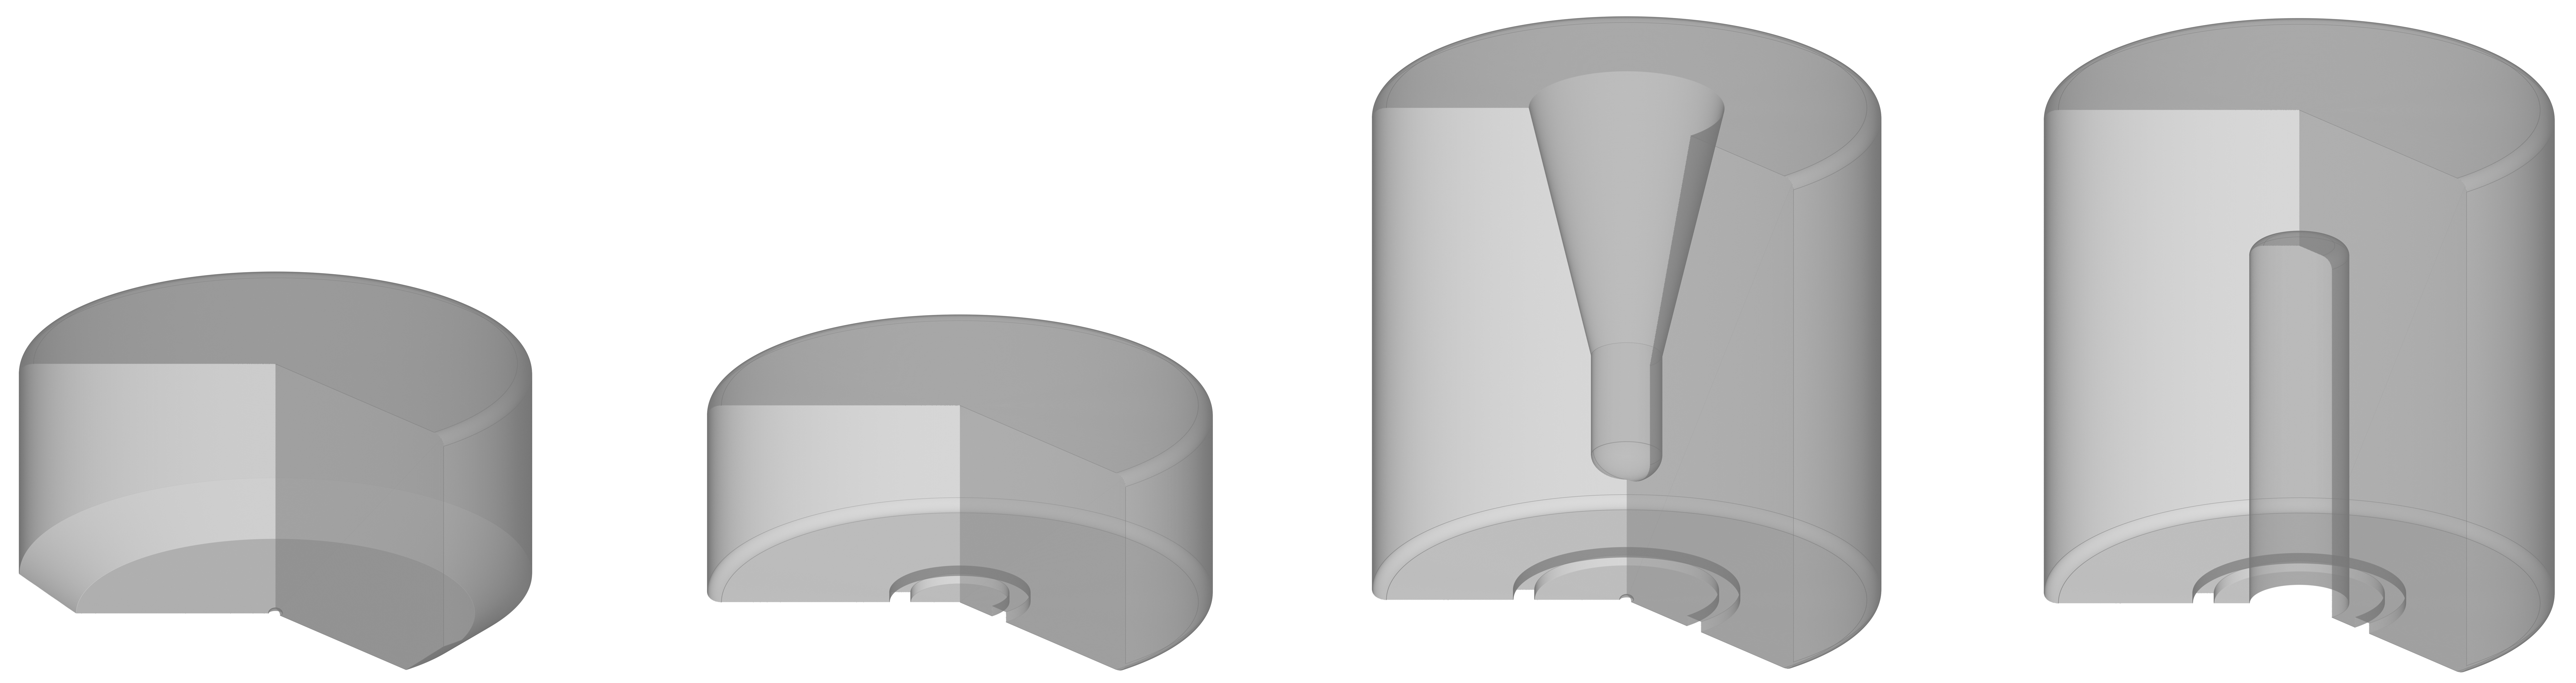
\includegraphics[width=6in]{figs/ge/detectors.png}
	\caption{PPC, ICPC, BEGe and semicoaxial bulk geometries.}
	\label{fig:det_geo}
\end{figure}
\begin{figure}[H]
	\centering
	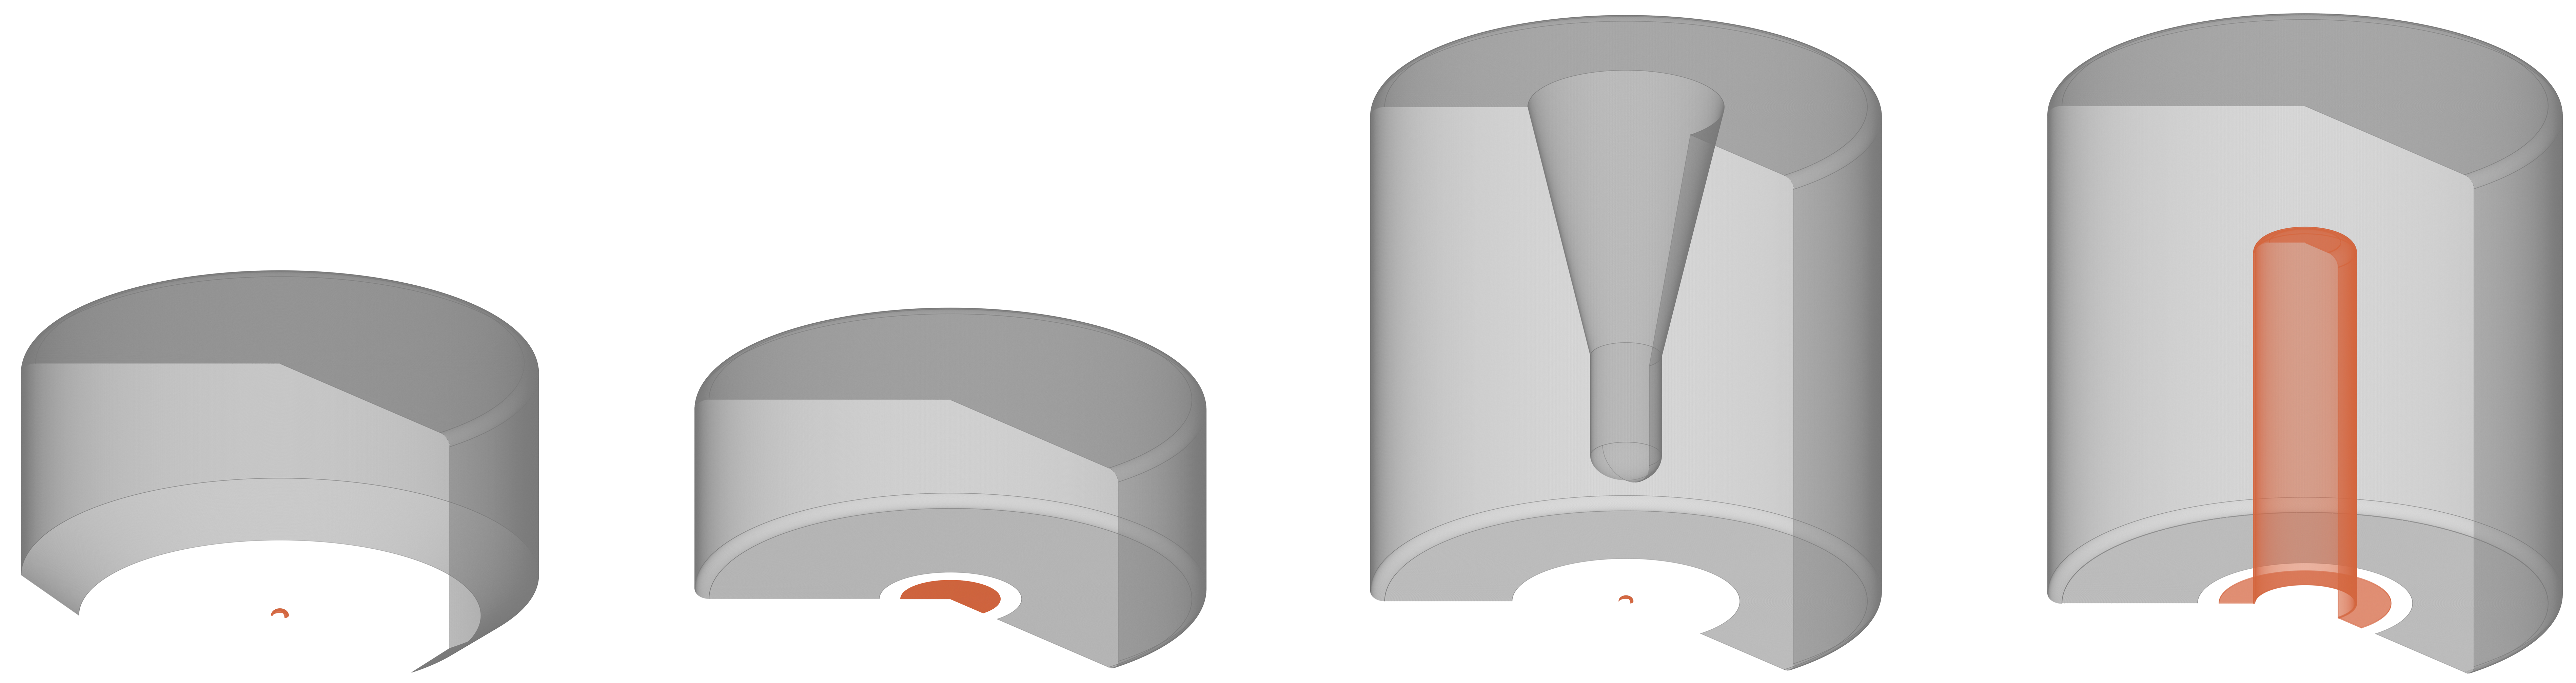
\includegraphics[width=6in]{figs/ge/contacts.png}
	\caption{PPC, ICPC, BEGe and semicoaxial contact geometries. The p$^+$ and n$^+$ contacts are depicted in orange and gray respectively. The surfaces depicted as empty are passivated.}
	\label{fig:det_contacts}
\end{figure}
\begin{figure}[H]
	\centering
	\subfigure[Electric field]{
		\centering
		\includegraphics[width = 2.9in]{figs/ge/e_field.png}
		\label{fig:dets_efield}
	}
	\subfigure[Weighting field]{
		\centering
		\includegraphics[width = 2.9in]{figs/ge/w_field.png}
		\label{fig:dets_weighting}
	}
	\caption{Electric and weighting fields of PPC, ICPC, BEGe and semicoaxial (from top to bottom) HPGe detectors. All detectors are biased 500\,V above the depletion voltage. Six contour lines are plotted for the weighting potential, corresponding to values given by $10^n$ where $n$ varies between -3.5 to -0.5 in steps of 0.5.} 
	\label{fig:dets_fields}
\end{figure}

\section{Energy Resolution}

To obtain a good energy resolution, the measured induced charge does not have to exactly match the charge created at event onset. Rather it just has to be consistent -- the induced charge should be the same for all events where the same charge was created. There are two stages where this consistency breaks down: charge collection and data acquisition. The first is discussed in Section~\ref{sec:charge_trapping}, where the amount of trapped charge varies on an event-by-event basis. The deviation in collected charge is proportional to the induced charge and cannot be fully eliminated by charge trapping corrections. The second is tied to the electronic noise introduced by the instrumentation required to amplify and record the signals. As discussed, detectors with large capacitance amplify this effect.

Of particular concern is low frequency noise, that is, noise with periods of the order or longer than the drift time. Although noise can be averaged or smoothed out, it comes at the cost of timing resolution. The result is that the timing resolution becomes limited to the period of the noise, rather than to the sampling period of the data acquisition apparatus. Thus, smoothing techniques are only applied to correct for high-frequency noise. If timing resolution is not a concern, such as in energy estimation, averaging over periods longer than the drift time through the use of filters is beneficial, and counteracts the effects of noise to an extent. Note that the effects of noise with periods longer than that of a recorded pulse can not be corrected with this method. The amplitude of the noise depends on the electronics circuit -- in which the detector plays the part of a capacitive element -- as a whole and is independent of the induced charge.

In the absence of noise and charge trapping the resolution of the detector is limited by the statistical nature of electron-hole pair production. Given a deposited energy $E_\text{dep}$, the ionization yield or number of electron-hole pairs created along track is $N = E_\text{dep}/\epsilon$. Recall that $\epsilon = 2.96$\,eV per electron-hole pair in Ge. If the number of impacts in the track were governed by a Poissonian distribution, the variance of the ionization yield -- \text{Var}(N)-- would be exactly $N$. Nevertheless, the variance measured by experiment is consistently lower than this value, leading to the conclusion that the events along the track are not independent. The Fano factor~\cite{fano}, $F$, accounts for the deviation from the Poisson predicted variance: $\text{Var}(N) = FE_\text{dep}/\epsilon$. The variance in the measured energy, E, is thus $\text{Var}(E) = \text{Var}(\epsilon N) = \epsilon^2\text{Var}(N) = F\epsilon E_\text{dep}$. In Ge the Fano factor was experimentally determined to be $F = 0.129 \pm 0.003$ at 77\,K~\cite{fanoGe}; however, considerable variation exists in literature. 

Summing the variance from the three effects described above, the resolution of a Ge detector can be parametrized by:
\begin{equation}
	\sigma(E) = \sqrt{\sigma_n^2 + \sigma_F^2E + \sigma_q^2E^2}~,
	\label{eq:energy_resolution}
\end{equation}
where $\sigma_n^2$ accounts for electronics noise, $\sigma_F^2E$ accounts for ionization yield statistics, including the Fano factor, and $\sigma_q^2E^2$ accounts for residual charge trapping. Note that $\sigma_F^2$ is left as a free parameter as opposed to explicitly using $F\epsilon$. This allows to account for energy calibration effects which relates $E$ to $E_\text{dep}$. 

In a hypothetical experiment which measures the ionization yield directly, the relative energy resolution is simply $\sigma/E = \sqrt{F\epsilon}$. Experiments using a wide range of detector technologies have been able to achieve energy resolutions which are dominated by this term, pointing to low noise and good ionization product collection. In this respect, Ge has a considerable advantage, given its comparably low Fano factor and high ionization yield (low $\epsilon$). In combination with its unprecedented high purity, low noise, well understood charge collection properties and modest active volume, the superb energy resolution of HPGe detectors makes them a great tool in the search for new physics.
